\nocite{Goodfellow-et-al-2016}

Konvolucijske neuronske mreže su posebna vrsta neuronskih mreža za obradu podataka koji imaju strukturu rešetke. Podaci koji su primjereni za obradu konvolucijskim mrežama mogu biti jednodimenzionalne rešetke, kao na primjer zvuk ili očitanja senzora u određenim vremenskim intervalima, dvodimenzionalne rešetke, kao što su slike, ili trodimenzionalne rešetke, kao što su video zapisi.
Ime konvolucijskih neuronskih mreža dolazi od matematičke operacije konvolucije koja se u njima koristi pa se i konvolucijske mreže mogu definirati kao neuronske mreže koje u barem jednom sloju umjesto množenja matrica koriste konvoluciju. U nastavku su opisane operacija konvolucije i operacija sažimanja, koja se u praksi često koristi zajedno s konvolucijom.

\subsection{Konvolucija}
Konvolucija je operacija nad dvije funkcije realne varijable. Kao primjer korištenja konvolucije možemo promatrati svemirski brod čiju lokaciju pratimo laserskim senzorom. Izlaz senzora je pozicija svemirskog broda u trenutku $t$ te ju označavamo s $x(t)$. Očitanje senzora možemo dobiti u bilo kojem trenutku t.
Pretpostavimo da su mjerenja senzora pokvarena šumom. Kako bi smanjili utjecaj šuma na očitanje, usrednjit ćemo nekoliko mjerenja s time da ćemo veću težinu dati mjerenju u trenutku $t$. To možemo postići funkcijom težine $w(a)$, gdje je $a$ starost mjerenja. Ako cjelobrojne takav težinski prosjek na mjerenje u svakom trenutku, dobijemo novu funkciju $s$ koja nam daje zaglađenu procjenu pozicije broda u trenutku $t$:
\[
s(t) = \int x(a)w(t-a)da
\]
Time smo definirali konvoluciju. Konvolucija se označava zvjezdicom:
\[
s(t) = (x \ast w)(t)
\]
U primjeru sa svemirskim brodom, $w$ mora biti funkcija gustoće vjerojatnosti da bi izlaz bio težinski prosjek. Također, $w$ mora biti jednak nuli za sve negativne argumente jer bismo u protivnom funkciji omogućili gledanje u budućnost za što je nemoguće dobiti podatke u promatranom trenutku. Općenito, konvolucija se može koristiti za razne primjene osim računanja težinskog prosjeka i definirana je za sve funkcije za koje je integral konvolucije definiran.
Kod konvolucijskih neuronskih mreža, funkciju $x$ zovemo ulaz, funkciju $w$ jezgra, a izlaz se naziva mapa značajki.
U primjeru svemirskog broda smo pretpostavili da je u svakom realnom trenutku $t$ moguće dobiti mjerenje senzora, međutim kod stvarnih mjerenja, podaci će biti dostupni u određenim vremenskim intervalima. Varijabla $t$ tada može poprimiti samo cjelobrojne vrijednosti pa možemo definirati diskretnu konvoluciju:
\[
s(t) = (x \ast w)(t) = \sum\limits_{a = - \infty}^{\infty} x(a)w(t-a) 
\] 
U velikom broju primjena neuronskih mreža, ulazi su višedimenzionalni nizovi (tenzori) podataka, a jezgre su u tom slučaju tenzori parametara. Budući da nemamo informacija o podacima koji nisu zapisani u ulaznim tenzorima, u većini slučajeva pretpostavljamo da su oni jednaki nuli, što nam olakšava implementaciju jer tada umjesto beskonačne sume trebamo izračunati sumu konačnog broja elemenata tenzora. U primjenama gdje su ulazni podaci višedimenzionalni, konvoluciju računamo istovremeno preko više osi, višedimenzionalnom jezgrom. Na primjer, kod slika imamo dvodimenzionalni ulaz pa koristimo i dvodimenzionalnu jezgru $K$. Konvoluciju tada računamo kao:
\[
S(i, j) = (I \ast K)(i, j) = \sum\limits_{m} \sum\limits_{n} I(m, n)K(i - m, j - n)
\]
Konvolucija je komutativna operacija pa se može zapisati i kao:
\[
S(i, j) = (I \ast K)(i, j) = \sum\limits_{m} \sum\limits_{n} I(i - m, j - n)K(m, n)
\]
čime smo jezgru okrenuli s obzirom na ulaz. 
Budući da u praksi komutativnost nije važno svojstvo, često se umjesto konvolucije koristi unakrsna korelacija ili neobrnuta konvolucija:
\[
S(i, j) = (I \ast K)(i, j) = \sum\limits_{m} \sum\limits_{n} I(i + m, j + n)K(m, n)
\]
U kontekstu strojnog učenja, optimizacijski algoritam će naučiti iste parametre jezgre ako koristi konvoluciju ili unakrsnu korelaciju samo na različitim mjestima. Za konvoluciju i unakrsnu korelaciju se često koristi zajednički naziv konvolucija. Slika \ref{konvolucija} prikazuje primjer izračuna unakrsne korelacije za dvodimenzionalni ulaz veličine $3 \times 3$ i dvodimenzionalnu jezgru veličine $2 \times 2$.

 \begin{figure}
	\centering
	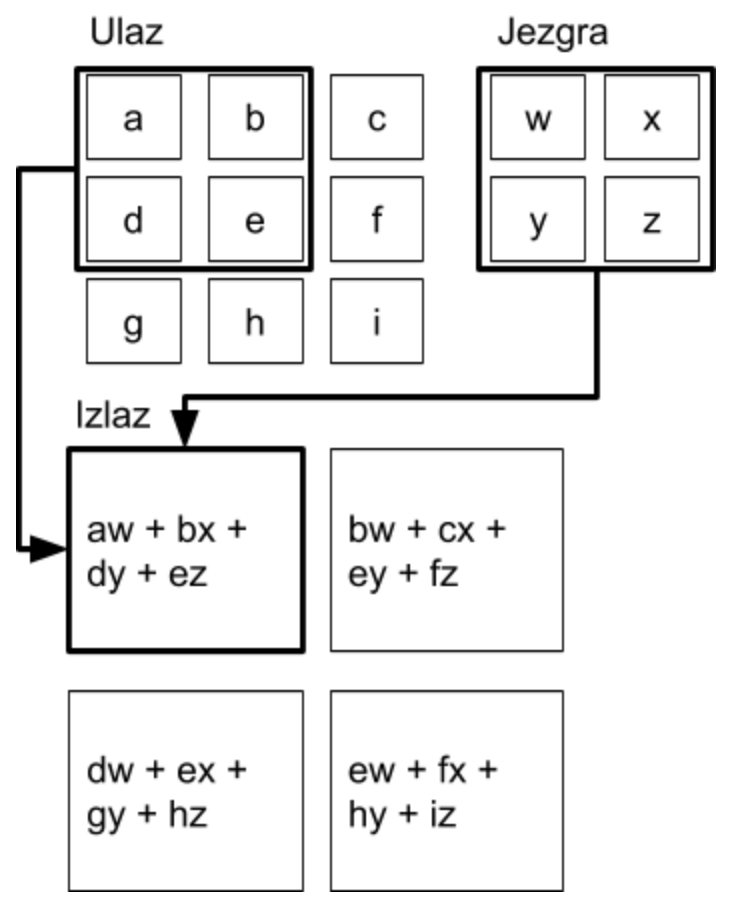
\includegraphics[scale=0.6]{img/konvolucija.png}
	\caption{Primjer konvolucije. Prozor veličine jezgre se pomiče po ulaznom tenzoru te se svaki element unutar prozora u ulaznom tenzoru množi s odgovarajućim elementom jezgre, a dobivene vrijednosti se zbrajaju. Za svaki pomak prozora se na izlazu dobije jedan broj.}
	\label{konvolucija}
\end{figure}

\subsection{Prednosti konvolucije}
Konvolucija koristi tri važne ideje koje poboljšavaju performanse neuronske mreže: rijetku povezanost, dijeljenje parametara i reprezentaciju ekvivarijantnu s obzirom na pomak. 
Slojevi potpuno povezanih neuronskih mreža množe matricu izlaza prethodnog sloja s matricom parametara gdje svaki element matrice parametara modelira vezu jednog ulaznog neurona s jednim izlaznim neuronom. To znači da ako prethodni sloj ima $m$ neurona, a trenutni $n$ parametara, matrica parametara trenutnog sloja mora biti dimenzija $m \times n$ i vremenska složenost izračuna izlaza sloja je $O(m \times n)$.
Za razliku od potpuno povezanih slojeva, konvolucijski slojevi su rijetko povezani, a to se postiže odabirom jezgre koja je manjih dimenzija od ulaza. Na primjer, slike mogu imati milijune piksela, a jezgra od nekoliko desetaka ili stotina piksela može biti dovoljna za naučiti korisne značajke. Ako broj veza izlaznog sloja ograničimo na $k$, gdje je $k \ll m$, prostorna i vremenska složenost će biti $O(k \times n)$. U praksi je moguće postići dobre rezultate koristeći $k$ koji je nekoliko redova veličine manji od $m$.
Dijeljenje parametara se odnosi na korištenje istih parametara za modeliranje više veza između ulaznih i izlaznih neurona. U potpuno povezanim slojevima, svaki težina se koristi samo jednom dok se kod konvolucijskih mreža svaki element jezgre koristi na svakoj poziciji ulaza. Dijeljenjem parametara postižemo da umjesto učenja novih parametara za svaku lokaciju ulaza, učimo samo jedan skup parametara što ne utječe na brzinu izvođenja, ali smanjuje broj parametara na $k$.
Rijetka povezanost i dijeljenje parametara omogućuju konvolucijskim mrežama rad s ulazima različitih veličina.
Razlike između potpuno povezanog sloja, rijetko povezanog sloja i rijetko povezanog sloja s dijeljenjem parametara ilustrirane su slikom \ref{povezanost}.
Posljedica dva opisana principa je svojstvo koje se zove ekvivarijantnost na pomak. Funkcija je ekvivarijantna ako se promjenom ulaza, izlaz mijenja na isti način, tj. ako vrijedi $f(g(x)) = g(f(x))$. Na primjer, neka je $I$ funkcija koja za zadane koordinate vraća svjetlinu slike i neka je $g$ funkcija koja pomiče svaki piksel slike za jedan u desno i vraća novu, translatiranu sliku $I' = g(I)$, gdje je $I'(x, y) = I(x-1, y)$. Napravimo li transformaciju $g$ na slici I i zatim nad dobivenom slikom primprimijenimojenimo konvoluciju, dobit ćemo isti rezultat kao da smo prvo primijenili konvoluciju nad slikom $I$, a zatim napravili transformaciju dobivenog izlaza. Svojstvo ekvivarijantnosti na pomak je korisno kada znamo da se slični ili isti uzorci mogu pojaviti na više mjesta u slici pa dijeljenje parametara omogućava da se jednom naučeni uzorci mogu prepoznati na bilo kojem mjestu u slici, bez obzira je li uzorak na tom mjestu viđen prilikom treninga ili nije. Primjer u kojem je ovo svojstvo važno je detekcija objekata. 
Konvolucija međutim nije ekvivarijantna s obzirom na skaliranje i rotaciju.

 \begin{figure}
	\centering
	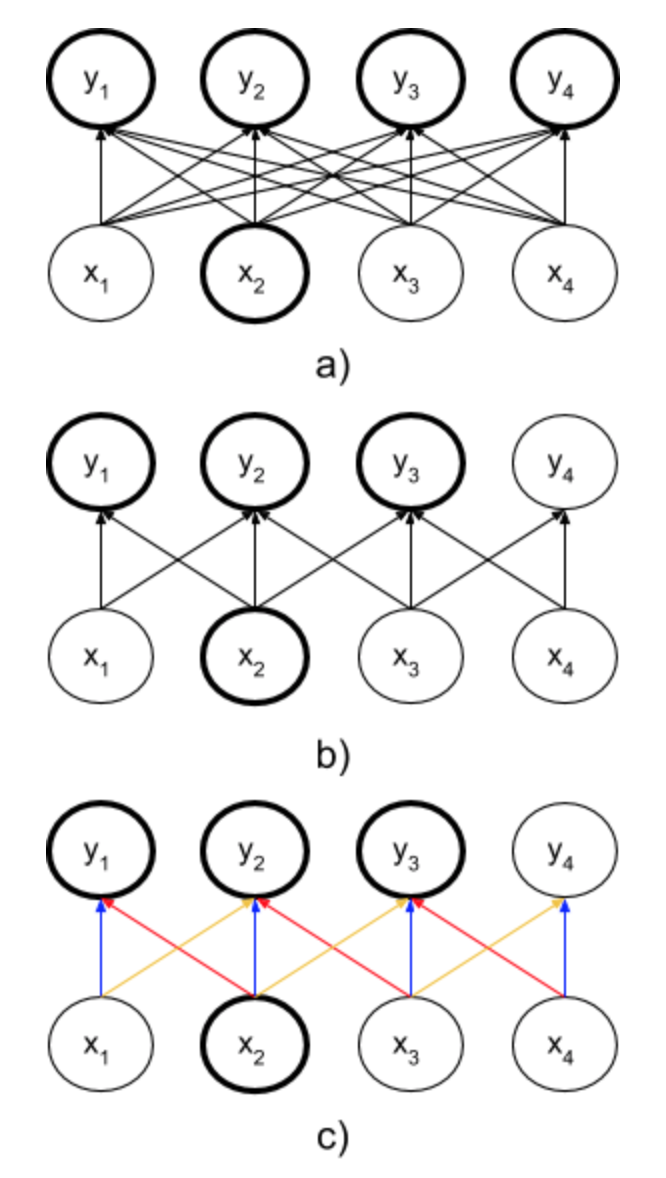
\includegraphics[scale=0.8]{img/povezanost.png}
	\caption{Slika a) prikazuje dva potpuno povezana sloja neuronske mreže. Svaki neuron u jednom sloju, povezan je sa svim neuronima drugog sloja. Težina veze između svaka dva neurona je poseban parametar pa zadani primjer ima 16 parametara. Slika b) prikazuje dva rijetko povezana sloja. Svaki neuron u jednom sloju je povezan samo s određenim brojem neurona u drugom sloju. Svaka veza dva neurona je poseban parametar pa je ukupan broj parametara 10. Slika c) prikazuje dva rijetko povezana sloja s dijeljenim parametrima. Veze između neurona označene istom bojom su isti parametri pa je ukupan broj parametara 3.}
	\label{povezanost}
\end{figure}

\subsection{Sažimanje}
Tipični konvolucijski sloj se sastoji od konvolucije, nelinearne aktivacijske funkcije i sloja sažimanja. Sloj sažimanja preslikava skup prostorno bliskih značajki na ulazu u jednu značajku na izlazu pri čemu je izlaz uglavnom neki statistički pokazatelj kao npr. srednja vrijednost ili maksimum. Općenito, sažimanjem se postiže invarijantnost na pomak što znači da ako se ulaz translatira za mali iznos, većina vrijednosti na izlazu sloja sažimanja će ostati nepromijenjena. Invarijantnost na male translacije je posebno korisna ako nas ne zanima točan položaj neke značajke, nego samo pojavljuje li se ta značajka ili ne. Budući da se sažimanjem dobije statistička mjera cijelog susjedstva, na izlazu možemo koristiti i manji broj značajki od samog broja ulaza. Kako bi se izbjeglo računanje izlaza koji se ne koriste, izlaze možemo računati tako da se pri računanju izlaza sloja sažimanja pomičemo za $k$ piksela umjesto za jedan. Time se postiže i veća brzina izvođenja jer se broj izračuna smanji za otprilike $k$ puta. Sažimanje je u mnogim primjenama važno za obradu ulaza različitih veličina. Na primjer, kod klasifikacije slika, potpuno povezani slojevi moraju imati fiksan ulaz pa se reguliranjem pomaka i veličine sloja sažimanja može osigurati da je izlaz iz sloja uvijek fiksne veličine. 

 \begin{figure}
	\centering
	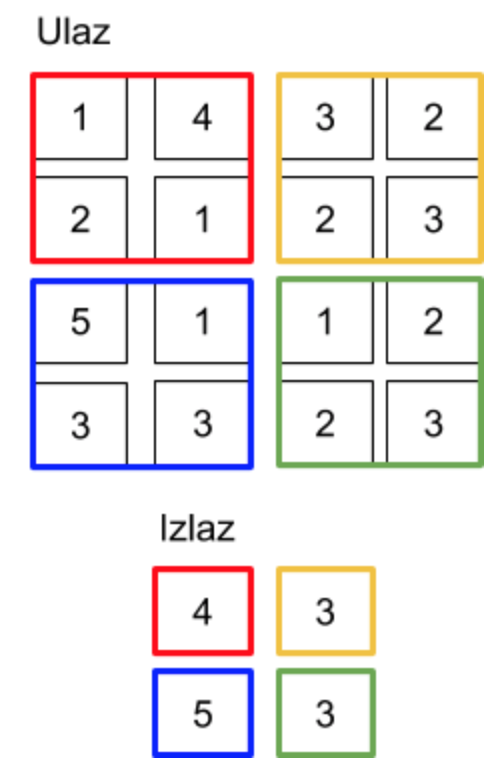
\includegraphics[scale=1]{img/sazimanje.png}
	\caption{Sažimanje maksimalnom vrijednosti s pomakom od 2 piksela.}
	\label{sazimanje}
\end{figure}